\section{Linear Displacement}
This algorithm is a simple but non-intuitive method to create fractal terrain. It is used as an example to model realistic planets\cite{paulbourke}, but can be easily be modified to generate rectangular heightmaps.
\subsection{Algorithm}
The approach of our algorithm can be summarized as following:
\bi
    \ib pick a random line going through the heightmap
    \ib  increase or decrease (decide at random) by one the height of each point under the line
    \ib repeat until you are satisfied with the result
\ei
These steps are shown in fig.~\ref{liter}, where we can see the algorithm at an increasing number of iterations.
The algorithm is suprisingly short, yet requires a great deal of iterations to get good results.
In our implementation the line is generated by choosing two random points in the grid and finding the equation of the line that passes through them.
In cartesian coordinates, if $(x_1,y_1)$ and $(x_2,y_2)$ are two independent random points with uniform distribution, then the equation of the line will be
\be
    \frac{y-y_1}{y_2-y_1}=\frac{x-x_1}{x_2-x_1}
\ee
The fact that we lift (or lower) all the points {\em under} this line is irrelevant and does not qualitatively change the terrain.
We could do it for the points {\em over} the line if we wanted to.
The original algorithm\cite{paulbourke}, raises one side and lowers the other, but this requires to access all points in the array at each iteration. 
Our method allows us to access on average only half of the array points, without losing any quality.

Finally a note on the number of iterations: to have a decent quality (no presence of artifacts), we usually need a number of iterations proportional to the number of points
\be\label{Niter}
    N_{iter} = q L_x L_y
\ee
where we define $0<q<1$ as the quality factor. To have acceptable results we empirically take $q\simeq 0.1$.
\subsection{Parallelization}
The parallelisation of this algorithm is quite simple, as the iterations do not depend on each other.
Therefore we split the number of iterations along the processes and, once that is complete, perform a {\tt MPI\_reduce()} to superpose the iterations of the different processes on the root process.

\begin{figure}[h]
\minipage{0.5\textwidth}
    \centering
    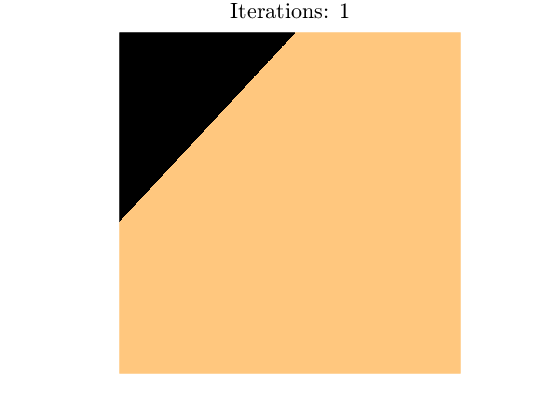
\includegraphics[width=\linewidth]{img/lines1.png}
\endminipage\hfill
\minipage{0.5\textwidth}
    \centering
    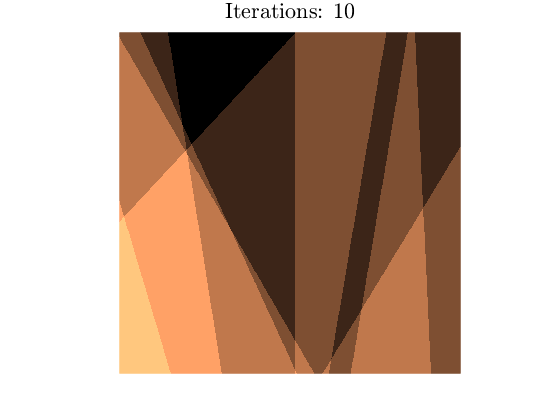
\includegraphics[width=\linewidth]{img/lines1e1.png}
\endminipage\hfill

\minipage{0.5\textwidth}
    \centering
    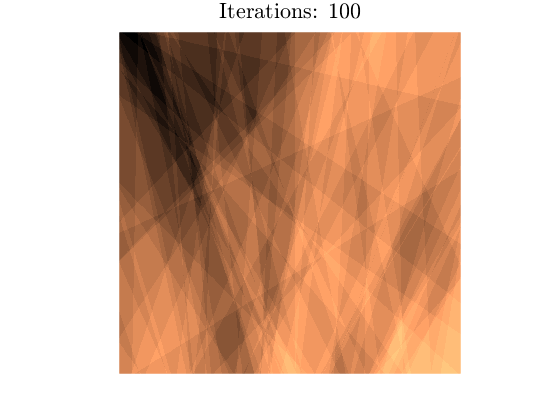
\includegraphics[width=\linewidth]{img/lines1e2.png}
\endminipage\hfill
\minipage{0.5\textwidth}
    \centering
    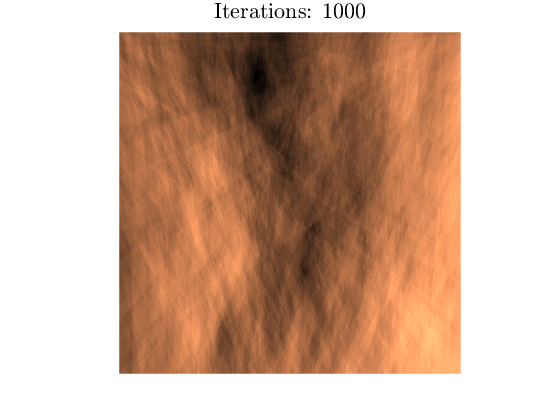
\includegraphics[width=\linewidth]{img/lines1e3.png}
\endminipage\hfill

\minipage{0.5\textwidth}
    \centering
    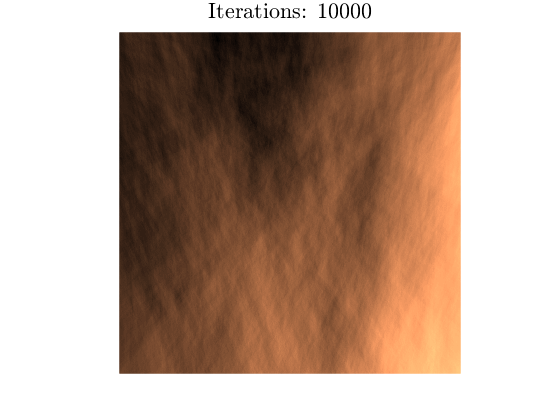
\includegraphics[width=\linewidth]{img/lines1e4.png}
\endminipage\hfill
\minipage{0.5\textwidth}
    \centering
    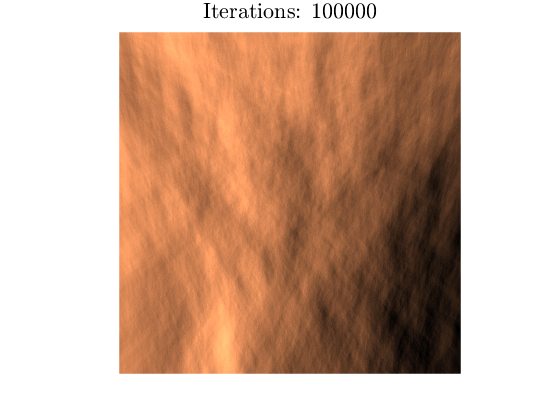
\includegraphics[width=\linewidth]{img/lines1e5.png}
\endminipage\hfill

\caption{\label{liter}Linear displacement algorithm with an increasing number of iterations.}
\end{figure}

\subsection{Performance analysis}
\subsubsection{Complexity}
For simplicity we assume $L = L_x = L_y$.
At each iteration we have to access on average $L^2/2$ points.
But, as discussed before, each process must perform $N_{iter}/N$ iterations.
Thus, by eq~\ref{Niter} we have a complexity of 
\be
    \underbrace{\order(q L^2/N) \order(L^2/2)}_{\text{iterations}} + \underbrace{\order(L^2\log{N})}_{\text{reduce}} = \underbrace{\order(L^4/N)}_{\text{overall}}
\ee
since we can safely assume that $N\ll L^2$. 

We remark that this algorithm is considerably slower as it does not scale as well as the other ones we present. However the constant hidden behind the $\order$ notation is considerably small --- we simply increment the value of a memory location --- making this algorithm  an interesting study case nonetheless.
\begin{figure}[htb]
\centering
    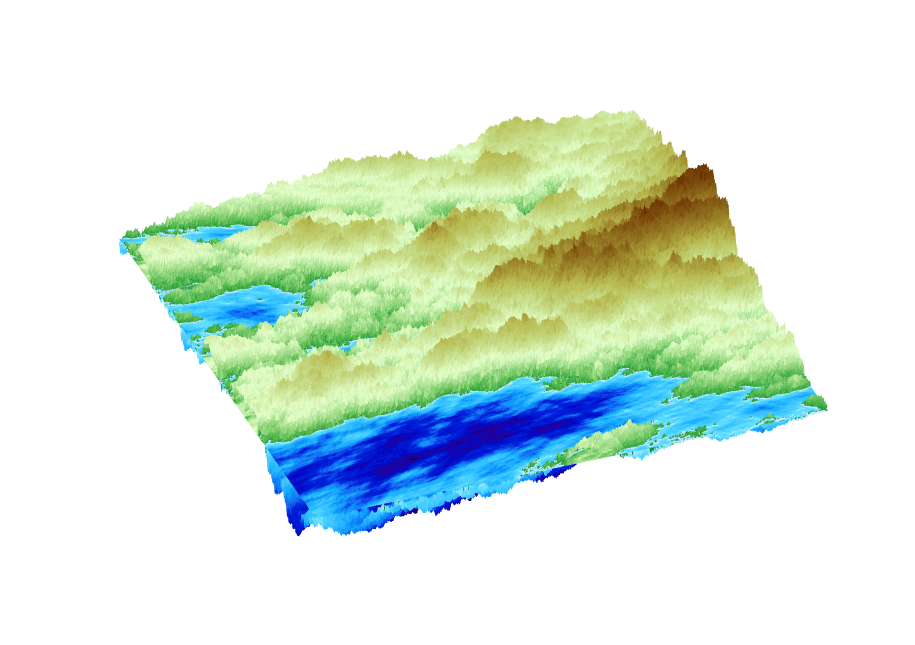
\includegraphics[width=0.8\textwidth]{img/lines3d.png}
    \caption{\label{lines3d}Example of terrain generated with the lines displacement algorithm}
\end{figure}

A tipical result is presented in fig.~\ref{lines3d}. We notice that the peaks are quite jagged. 
One feature of this algorithm is that it does not take any parameter to control the ``smoothness'' of the fractal.

\subsubsection{Experimental results}

Runs on the {\em Ferlin} computer at PDC confirm that this algorithm is significantly slower than the other two presented. For this reason the benchmarking has been done with significantly lower sizes.

\begin{figure}[!htb]
\minipage{0.5\textwidth}
    \centering
    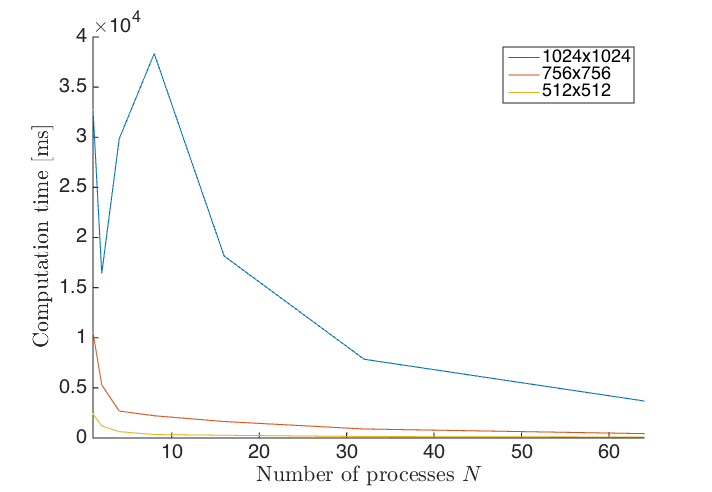
\includegraphics[width=\linewidth]{img/lines_benchmarks1.png}
    \caption{Execution time for the linear displacement algorithm}
    \label{fig:benchmarks_time_ld}
\endminipage\hfill
\minipage{0.5\textwidth}
    \centering
    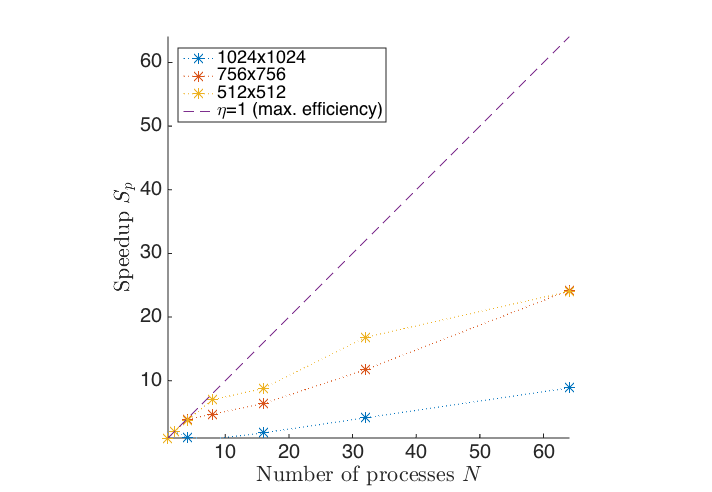
\includegraphics[width=\linewidth]{img/lines_benchmarks2.png}
    \caption{Speedup for the linear displacement algorithm}
    \label{fig:benchmarks_speedup_ld}
\endminipage\hfill
\end{figure}

By inspecting the performance results in fig.~\ref{fig:benchmarks_time_ld} and fig.~\ref{fig:benchmarks_speedup_ld} we see that the performance is very sensitive to the number of processes and the efficiency actually goes down with the size of the height map.
This suggest that the major bottleneck is the communication step, where the processes communicate a very large amount of data.

The data collected is summarized in table~\ref{table:speedup_ld}, along with the average speedup.

\begin{table}[H]
\begin{center}
\begin{tabular}{c|c|c|c|c|}
$L$ =  & 512 & 756 & 1024 &  \\
\hline
Processes & \multicolumn{3}{c|}{$T_p$ [s]} & {$\bar{S_p}$} \\
\hline
$2$ & 1.2160 & 5.2860 & 16.4160 & 1.98\\
$4$ & 0.6330 & 2.6900 & 29.8530 & 2.94\\
$8$ & 0.3430 & 2.2200 & 38.3460 & 4.20\\
$16$ & 0.2730 & 1.6430 & 18.1460 & 5.67\\
$32$ & 0.1430 & 0.9000 & 7.8560 & 10.9\\
$64$ & 0.1000 & 0.4360 & 3.6960 & 19.0\\

\hline
\end{tabular}
\caption{\label{table:speedup_ld} Running time $T_p$ and average speedup $\bar{S_p}$ for different amount of processes and sizes.}
\end{center}
\end{table}




    